\documentclass{article}
\usepackage[utf8]{inputenc}
\usepackage{graphicx}

\title{Leap Year}

\begin{document}

\maketitle

\section{Leap year explanation}

\begin{figure}
    \centering
    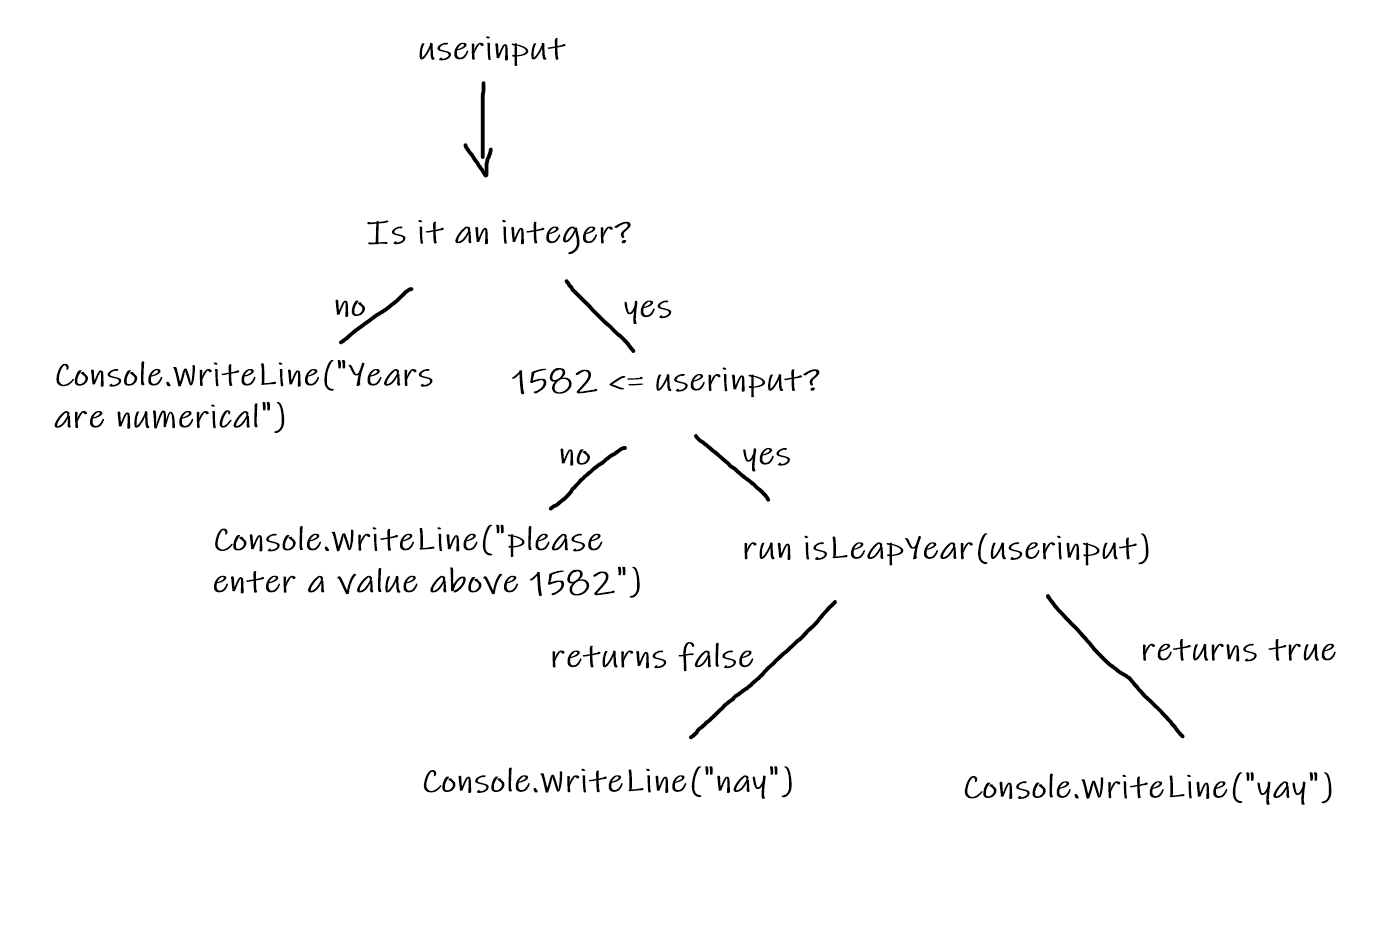
\includegraphics[width=\textwidth]{Leap_Year.png}
    \caption{Drawing of my leap year implementation}
    \label{fig:my_label}
\end{figure}
    
First the program receives a user input. This input is then checked whether or not it is a valid input (an integer in this case), and will respond accordingly. If it is not an integer, it will stop here with a print statement, else it will move on, and check whether the input is at least 1582. If it is not, it will stop with a user input, else it will run the isLeapYear() function. This function returns a boolean which is dependent on whether the user input is a leap year or not. The function calculates this by checking that the given number is either divisible by 400 or divisible by 4 AND not divisible by 100. The final print statement is then dependent on this boolean, and will write yay if it is true, and nay if it is false.
\end{document}
